\documentclass[12pt]{amsart}

\usepackage{mathrsfs, fullpage, amsmath, amssymb, graphicx, xcolor, tikz}

\renewcommand{\phi}{\varphi}
\renewcommand{\epsilon}{\varepsilon}
\renewcommand{\hat}{\widehat}
\newcommand{\bx}{\boldsymbol{x}}
\newcommand{\by}{\boldsymbol{y}}
\newcommand{\cA}{\mathscr{A}}
\newcommand{\cB}{\mathscr{B}}
\newcommand{\cC}{\mathscr{C}}
\newcommand{\cD}{\mathscr{D}}
\newcommand{\cF}{\mathscr{F}}
\newcommand{\cG}{\mathscr{G}}
\newcommand{\cN}{\mathscr{N}}
\newcommand{\cO}{\mathscr{O}}
\newcommand{\cP}{\mathscr{P}}
\newcommand{\cX}{\mathscr{X}}
\newcommand{\cY}{\mathscr{Y}}
\newcommand{\PP}{\mathbb{P}}
\newcommand{\RR}{\mathbb{R}}
\newcommand{\ZZ}{\mathbb{Z}}
\newcommand{\lra}{\longrightarrow}
\newcommand{\One}{\mathbf{1}}
\newcommand{\blank}{\,\cdot\,}

\newcommand{\vpi}{\boldsymbol{\pi}}
\newcommand{\vtheta}{\boldsymbol{\theta}}
\newcommand{\ve}{\boldsymbol{e}}
\newcommand{\vu}{\boldsymbol{u}}
\newcommand{\vv}{\boldsymbol{v}}
\newcommand{\vw}{\boldsymbol{w}}
\newcommand{\vx}{\boldsymbol{x}}
\newcommand{\vy}{\boldsymbol{y}}
\newcommand{\vz}{\boldsymbol{z}}
\newcommand{\vZ}{\boldsymbol{Z}}

\newcommand{\xhat}{\hat{x}}
\newcommand{\yhat}{\hat{y}}
\newcommand{\bxhat}{\hat{\bx}}
\newcommand{\byhat}{\hat{\by}}
\newcommand{\betahat}{\hat{\beta}}

\newcommand{\iid}{i.i.d.\ }

\DeclareMathOperator{\Bias}{Bias}
\DeclareMathOperator{\EE}{E}
\DeclareMathOperator{\Cov}{Cov}
\DeclareMathOperator{\cov}{cov}
\DeclareMathOperator{\Var}{Var}
\DeclareMathOperator{\Mult}{Mult}
\DeclareMathOperator{\Ber}{Ber}
\DeclareMathOperator{\var}{var}
\DeclareMathOperator{\mean}{mean}
\DeclareMathOperator{\MSE}{MSE}
\DeclareMathOperator{\SSE}{SSE}
\DeclareMathOperator{\ESS}{ESS}
\DeclareMathOperator{\RSS}{RSS}
\DeclareMathOperator{\TSS}{TSS}
\DeclareMathOperator{\argmin}{argmin}
\DeclareMathOperator{\Argmin}{\mathop{\argmin}}


\newtheorem{theorem}{Theorem}
\newtheorem{lemma}[theorem]{Lemma}
\newtheorem{thmdef}[theorem]{Theorem-Definition}

\setlength\parskip{1em}
\setlength\parindent{0em}

\definecolor{orange}{HTML}{FF7F0E}
\definecolor{green}{HTML}{2CA02C}
\definecolor{blue}{HTML}{1F77B4}

\DeclareRobustCommand\orangeline{\raisebox{0.5ex}{\tikz \draw[orange, thick] (1, 0) -- (0.5, 0);}}
\DeclareRobustCommand\blueline{\raisebox{0.5ex}{\tikz \draw[blue, thick] (1, 0) -- (0.5, 0);}}

\begin{document}
\section{Simple linear regression}

\subsection{The regression line}
Consider a data set
\[
    \cD=\{(x_i, y_i):i=1,\ldots,n\}.
\]
If the \emph{mean-squared error} function
\[
    \MSE(a,b) = \frac1n\sum_{i=1}^n (a x_i + b - y_i)^2
\]
achieves its absolute minimum value at \[(a,b)=(\alpha, \beta)\] then the line $y=\alpha x+\beta$
is called the \emph{regression line} or \emph{least-squares line} for $\cD$.

The \emph{slope}, $\alpha$, and the \emph{intercept}, $\beta$ of the regression line (its \emph{coefficients}) can be expressed
in terms of basic statistics of $\cD$:
\begin{align*}
    \text{means:}& &\bar{x} &= \frac1n\sum_{i=1}^n x_i,& \bar{y} &= \frac1n\sum_{i=1}^n y_i\\
    \text{variances:}& &s_x^2 &= \frac1n\sum_{i=1}^n (x_i - \bar{x})^2,& s_y^2 &= \frac1n\sum_{i=1}^n (y_i-\bar{y})^2\\
    \text{covariance:}& &s_{xy} &= \frac1n\sum_{i=1}^n (x_i - \bar{x})(y_i-\bar{y})
\end{align*}

\begin{theorem}[Gauss/Legendre]\label{T:GaussLegendre}
The coefficients of the regression line of $\cD$ are:
\[
    a=\frac{s_{xy}}{s_x^2},\qquad b=\bar y = a\bar x.
\]
\end{theorem}
\begin{proof}
    Notice that
    \[
        \min_{(a,b)}
        \MSE(a,b) = \min_a\left(\min_b\MSE(a,b)\right).
    \]
    For a given $a$, the quantity $\MSE(a, b)$ is a quadratic polynomial in $b$:
    \[
        \MSE(a, b)=b^2 - 2\left(\frac1n\sum_{i=1}^n(y_i-ax_i)\right)b + \sum_{i=1}^n(y_i-ax_i)
    \]
    Since a quadratic polynomial $t^2-2qt+r$ achieves its minimum value at $t=q$,
    $\MSE(a, b)$ achieves its minimum value when
    \[
        b=\frac1n\sum_{i=1}^n(y_i-ax_i) = \bar{y}-a\bar{x}.
    \]

    It remains to determine
    \[
        \min_a\MSE(a, \bar y - a\bar x)
        =\min_a \frac1n\sum_{i=1}^n (ax_i + (\bar{y}-a\bar{x}) - y_i)^2.
    \]
    Expanding and rearranging, we get
    \[
        \frac1n\sum_{i=1}^n (ax_i + (\bar{y}-a\bar{x}) - y_i)^2 = s_x^2 a^2 - 2s_{xy}a + s_y^2.
    \]
    Since a quadratic polynomial $pt^2-2qt+r$ achieves its minimum value at $t=q/p$,
    the function $\MSE(a, \bar y - a\bar x)$ achieves its minimum value when $a=s_{xy}/s_x^2$.
    
    Thus, $\MSE(a, b)$ is minimized when
    \[
        a=\frac{s_{xy}}{s_x^2},\qquad b=\bar y - a\bar x.\qedhere
    \]
\end{proof}

Define $\One$, $\vx$, $\vy\in\RR^n$ by
\[
    \One= \begin{pmatrix}
        1\\\vdots\\1
    \end{pmatrix},\quad
    \vx= \begin{pmatrix}
        x_1\\\vdots\\x_n
    \end{pmatrix},\quad
    \vy= \begin{pmatrix}
        y_1\\\vdots\\y_n
    \end{pmatrix}.
\]
For $\alpha$, $\beta\in\RR$, define the associated \emph{residual vector}, $\ve(\alpha,\beta)$, by
\[    
    \ve(\alpha,\beta)=\alpha\vx + \beta\One - \vy.
\]
Then
\[
    \MSE(\alpha,\beta) = \frac1n\|\ve(\alpha,\beta)\|^2.
\]
Let $U$ be the subspace of $\RR^n$ spanned by the vectors $\vx$ and $\One$:
\[
U = \{\alpha\vx + \beta\One: \alpha,\beta\in\RR^n\}.
\]
Let $d(\vy, U)$ be the distance from $\vy$ to $U$, i.e.,
the minimal distance from $\vy$ to an element of $U$:
\[
    d(\vy, U) = \inf_{a,b}\|a\vx + b\One - \vy\|.
\]
The infimum on the right is achieved by \emph{orthogonal projection of $\vy$ onto $U$,} i.e.,
the unique vector $\hat\vy\in U$ such that
\[
    \langle\hat\vy, \vy-\hat\vy\rangle=0.
\]
If $\{\vu_1,\vu_2\}$ is any orthonormal basis of $U$, then
\[
    \hat\vy = \langle\vu_1,\vy\rangle\vu_1 + \langle\vu_2,\vy\rangle\vu_2. 
\]
We can construct an orthonormal basis of $U$ be applying the
\emph{Gram-Schmidt orthonormalization procedure} to the spanning set $\{\One,\vx\}$.
Let
\begin{align*}
    \vu_1 &= \frac1{\|\One\|}\One = \frac1{\sqrt n}\One,\\
    \vu_2' &= \vx - \langle\vu_1, \vx\rangle\vu_1\\
    &= \vx - \frac1{\sqrt n}\langle\One,\vx\rangle\frac1{\sqrt n}\One\\
    &= \vx - \bar x\One,\\
    \intertext{Assume that $\bx$ and $\One$ are linearly independent. Then $\vu_2'\neq 0$ and we may set}
    \vu_2 &= \frac1{\|\vu_2'\|}\vu_2'\\
    &= \frac1{\sqrt n s_x}(\vx - \bar x\One)
\end{align*}
Thus, if $\bx$ and $\One$ are linearly independent, then
\[
    \left\{\frac1{\sqrt n}\One,\; \frac1{\sqrt n s_x}(\vx - \bar x\One)\right\}.
\]
is an orthonormal basis of $U$.
It follows that
\[
    \hat\vy = \frac1n\left\langle \One, \vy\right\rangle\One + 
    \frac1{n s_x^2}\left\langle\vx - \bar x\One,\vy\right\rangle (\vx - \bar x\One)
\]
Since $\vx-\bar x\One$ is orthogonal to $\One$,
\[
    \frac1n\left\langle\vx - \bar x\One,\vy\right\rangle = \frac1n\left\langle\vx - \bar x\One,\vy - \bar y\One\right\rangle = \frac1n\sum_{i=1}^n(x_i-\bar x)(y_i-\bar y) = s_{xy}.
\]
\[
    \hat \vy = \bar y\One + \frac{s_{xy}}{s_x^2}(\vx-\bar x\One) = \frac{s_{xy}}{s_x^2}\vx + \left(\bar y - \frac{s_{xy}}{s_x^2}\bar x\right)\One
\]
\begin{theorem}\hfill
    \begin{enumerate}
        \item There is a unique vector $\hat\vy\in U$ such that 
    \[d(\vy, U) = \|\vy-\hat\vy\|.\]
    \item If the vectors $\One$ and $\vx$ are linearly independent,
    then there are unique scalars $\hat a$ and $\hat b$ such that
    \[\hat\vy = \hat a\vx + \hat b\One.\]
\end{enumerate}
\end{theorem}

\[
    \| \vy - \bar y\One\|^2 = \| (\vy - \hat{\vy})  + (\hat\vy - \bar y\One)\|^2 = \|\vy - \hat \vy\|^2 + \|\hat \vy - \bar y\One\|^2 = \SSE + s_{\hat \vy}^2
\]

\subsection{Sums of squares}
The regression line gives the estimate
\[
    \hat{y}_i = ax_i + b
\]
for $y_i$. The $\hat{y}_i$ and the $y_i$ have the same mean:
\[
    \overline{\hat y} = \frac1n\sum_{i=1}^n \hat{y}_i =\frac1n\sum_{i=1}^n(ax_i + b) =  a\bar{x} + b = \bar{y},
\]
the final equality following from Theorem~\ref{T:GaussLegendre}.

\begin{align*}
s_y^2 &= \frac1n\sum_{i=1}^n (y_i - \bar y)^2\\
&= \frac1n\sum_{i=1}^n (y_i - \hat{y}_i + \hat{y}_i - \bar y)^2\\
&= \frac1n\sum_{i=1}^n (y_i - \hat{y}_i)^2 
+ 2\frac1n\sum_{i=1}^n (y_i - \hat{y}_i)(\hat{y}_i - \bar y)
+ \frac1n\sum_{i=1}^n(\hat{y}_i - \bar y)^2\\
&= \MSE(a, b) + 2s_{e\hat{y}} + s_{\hat{y}}^2.
\end{align*}

\section{The bivariate normal distribution}

The bivariate normal density with means $\mu_1$ and $\mu_2$, variances $\sigma_1$ and $\sigma_2$,
and correlation $\rho$ is defined by
\[
f(x_1, x_2) 
= \frac1{2\sigma_1\sigma_2\sqrt{1-\rho^2}}e^{-\frac1{2}Q(x_1, x_2)},
\]
where
\[
    Q(x_1,x_2) = \frac1{\sqrt{1-\rho^2}}\left[
    \left(\frac{x_1-\mu_1}{\sigma_1}\right)^2
    - 2\rho \left(\frac{x_1-\mu_1}{\sigma_1}\right)\left(\frac{x_2-\mu_2}{\sigma_2}\right)
    + \left(\frac{x_2-\mu_2}{\sigma_2}\right)^2\right]
\]
We write
\[
    (X_1,X_2)\sim N(\mu_1, \mu_2, \sigma_1, \sigma_2, \rho)
\]
if $(X_1,X_2)$ has density $f(x_1,x_2)$. 

Suppose $X\sim N(\mu_1, \mu_2, \sigma_1, \sigma_2, \rho)$. Prove:
\begin{enumerate}
    \setlength{\itemsep}{1em}
    \item The marginal density of $X_1$ is the univariate normal density with mean $\mu_1$ 
    and variance $\sigma_1^2$, i.e.,
    $$\int_{-\infty}^\infty f(x_1,x_2)\,dx_2 = \frac1{\sqrt{2\pi}\sigma_1}
    e^{-\frac12\left(\frac{x_1-\mu_1}{\sigma_1}\right)}.$$
    \item $\EE[X_i]=\mu_i$, $\EE[(X_i - \mu_i)^2]=\sigma_i^2$, and 
    $\EE[(X_1-\mu_1)(X_2-\mu_2)]=\sigma_1\sigma_2\rho$.
    \item The conditional density of $X_2$ given $X_1$ is given by
    $$
    f(x_2|x_1) = \frac1{\sqrt{2\pi(1-\rho^2)}\sigma_2}e^{-\frac12\left(\frac{x_2-\left(\rho\frac{\sigma_2}{\sigma_1}(x_1-\mu_1) + \mu_2\right)}{\sqrt{1-\rho^2}\sigma_2}\right)^2}.
    $$
\item The conditional expectation and variance of $X_2$ given $X_1$ are given by
    $$
    \EE[X_2|X_1] = \rho\frac{\sigma_2}{\sigma_1}(X_1-\mu_1) + \mu_2
    $$
    and
    $$
    \EE[(X_2 - \EE[X_2|X_1])^2|X_1] = \sqrt{1-\rho^2}\sigma_2,
    $$
    respectively.
    Note that the latter quantity is independent of $X_1$.
\end{enumerate}

\section{Conditional Expectation}
\begin{thmdef}
Let $\Omega$ be a set equipped with a probability measure, $P$.
Given random variables $X$ and $Y$ on $\Omega$, there is a unique function
$f:\RR\to\RR$ such that
\[
    \int_{[X\in G]}Y\,dP = \int_{[X\in G]}f(X)\,dP,
\]
for every $E\subseteq \RR$. The random variable $f(X)$ is called the
\emph{conditional expectation of $Y$ given $X$} and denoted $\EE[Y|X]$.
\end{thmdef}

\begin{enumerate}
    \setlength{\itemsep}{1em}
    \item If $Y=f(X)$, then $\EE[Y|X]=Y$.
    \item If $X=1$, then $\EE[Y|X]=\EE[Y]$:
\begin{align*}
    1\notin G:& & &\int_{[X\in G]} Y\,dP = \int_{\varnothing}Y\,dP = 0 = \int_{\varnothing}\EE[Y]\,dP = \int_{[X\in G]} \EE[Y]\,dP\\[0.5em]
    1\in G:& & &\int_{[X\in G]} Y\,dP = \int_\Omega Y\,dP = \EE[Y] = \int_\Omega \EE[Y]\,dP = \int_{[X\in G]} \EE[Y]\,dP
\end{align*}
\item If $\EE[Y|X]=f(X)$, then $$\EE[I_H(X)Y|X]=I_H(X)f(X)$$ for all $H\subseteq\RR$:
\begin{align*}
\int_{[X\in G]} I_H(X)Y\,dP =     \int_{[X\in G\cap H]} Y\,dP = \int_{[X\in G\cap H]} f(X)\,dP = \int_{[X\in G]} I_H(X)f(X)\,dP
\end{align*}
\item If $u:\RR\to\RR$, then $$\EE[u(X)Y|X]=u(X)\EE[Y|X].$$
(Proof: Exercise?)
\item If $X=u(Y)$, then $$\EE[\EE[Z|Y]|X]=\EE[Z|X].$$
\begin{align*}
    \int_{[u(X)\in G]} \EE[Y|X]\,dP &=
    \int_{[X\in u^{-1}(G)]} \EE[Y|X]\,dP\\
    &= \int_{[X\in u^{-1}(G)]} Y\,dP\\
    &= \int_{[u(X)\in G]} Y\,dP\\
    &= \int_{[u(X)\in G]} \EE[Y|u(X)]\,dP\\
\end{align*}
\end{enumerate}
Exercise: $X$ has countable range...

\begin{lemma}
    $\Cov(u(X), Y-\EE[X])=0$.
\end{lemma}
\begin{proof}
    \[\Cov(u(X), Y-E[Y|X]) = \EE[u(X)\EE[Y|X]]\]
\end{proof}

\begin{align*}
    \EE[(Y - f(X))^2] &= \EE[(Y - \EE[Y|X] + \EE[Y|X] - f(X))^2]\\
    &= \EE[(Y - \EE[Y|X])^2] + 2\Cov(Y-\EE[Y|X], E[Y|X] - f(X)) + \EE[f(X)^2]
\end{align*}

\begin{lemma}
    The following are equivalent:
    \begin{enumerate}
        \setlength{\itemsep}{1em}
        \item $\EE[Y|X]=Y$
        \item $Y=f(X)$ for some $f:\RR\to\RR$.
        \item $\Cov(Y, Z-\EE[Z|X])=0$ for all random variables $Z$.
    \end{enumerate}
\end{lemma}
\begin{proof}\hfill
    \begin{enumerate}
        \item[$(1)\Rightarrow(2)$] $\EE[Y|X]$ is, by definition, a function of $X$.
        \item[$(2)\Rightarrow(3)$] We have:
        \begin{align*}
            \Cov(f(X), Z-\EE[Z|X])
            &= \EE[f(X)(Z-\EE[Z|X])]\\
            &= \EE[f(X)Z] - \EE[f(X)\EE[Z|X]]\\
            &= \EE[f(X)Z] - \EE[\EE[f(X)Z|X]]\\
            &= \EE[f(X)Z] - \EE[f(X)Z]\\
            &= 0.
        \end{align*}
        \item[$(3)\Rightarrow(1)$] 
    \end{enumerate}
\end{proof}


\begin{align*}
    \EE[u(X)Y] &= \EE[\EE[u(X)Y|X]]\\
    &=\EE[u(X)\EE[Y|X]]\\
\end{align*}

Let $f(x,y)$ be the empirical density associated to the data set 
$(x_1,y_1),\ldots,(x_n, y_n)$:
\[
    f(x,y) = \frac1n\sum_{i=1}^n \delta(x - x_i)\delta(y - y_i)
\]
Suppose that $(X,Y)$ has joint density $f(x,y)$.
The marginal densities $f(x)$ and $f(y)$ of $X$ and $Y$ are
\[
    f(x) =  \frac1n\sum_{i=1}^n\delta(x - x_i)\quad\text{and}\quad
f(y) = \frac1n\sum_{i=1}^n\delta(y - y_i).
\]
Let's project $Y-\EE Y$ onto the span of the uncorrelated random variables $1$ and $X-\EE X$.
It's easy to show (exercise) that $\EE X=\bar x$ and $\EE Y = \bar y$.
\[
    \bar x := \frac1n\sum_{i=1}^n x_i\qquad\text{and}\qquad
    \bar y = \frac1n\sum_{i=1}^n y_i,
\]
Therefore,
\begin{align*}
    \EE[(X - \EE X)(Y - \EE Y)] &= \iint (y-\bar y)(x - \bar x)f(x,y)\,dx\,dy\\
    &= \frac1n\sum_{i=1}^n(x_i - \bar x)(y_i - \bar y) = \cov(x, y).
\end{align*}
Obviously,
\[
    \EE[1(Y-\EE Y)] = 0.
\]
Therefore, the projection of $Y - \EE Y$ onto the span of $1$ and $X - \EE X$ is
\[\frac{\EE[1(Y - \EE Y)]}{\EE[1^2]} 1 + \frac{\EE[(X-\EE X)(Y - \EE Y)]}{\EE[(X-\EE X)^2]}(X - \EE X) = \frac{\cov(x,y)}{\var(x)}(X-\bar x)\]
It follows that the linear regression of $Y$ on $X$ is
\[
\hat Y = \frac{\cov(x,y)}{\var(x)}(X-\bar x) + \bar y
\]

Consider the probability space \[(\RR^2, f(x,y)\,dx\,dy),\] where $f(x,y)$ is the \emph{empirical density}
associated to the data set $(x_1,y_1),\ldots,(x_n, y_n)$:
\[
    f(x,y) = \frac1n\sum_{i=1}^n \delta(x - x_i)\delta(y - y_i).
\]
Let
\[
    V := L^2(\RR^2, f(x,y)\,dx\,dy) = \left\{Z:\RR^2\to \RR : \iint |Z(x,y)|^2f(x,y)\,dx\,dy\right\}
\]
\begin{figure}
    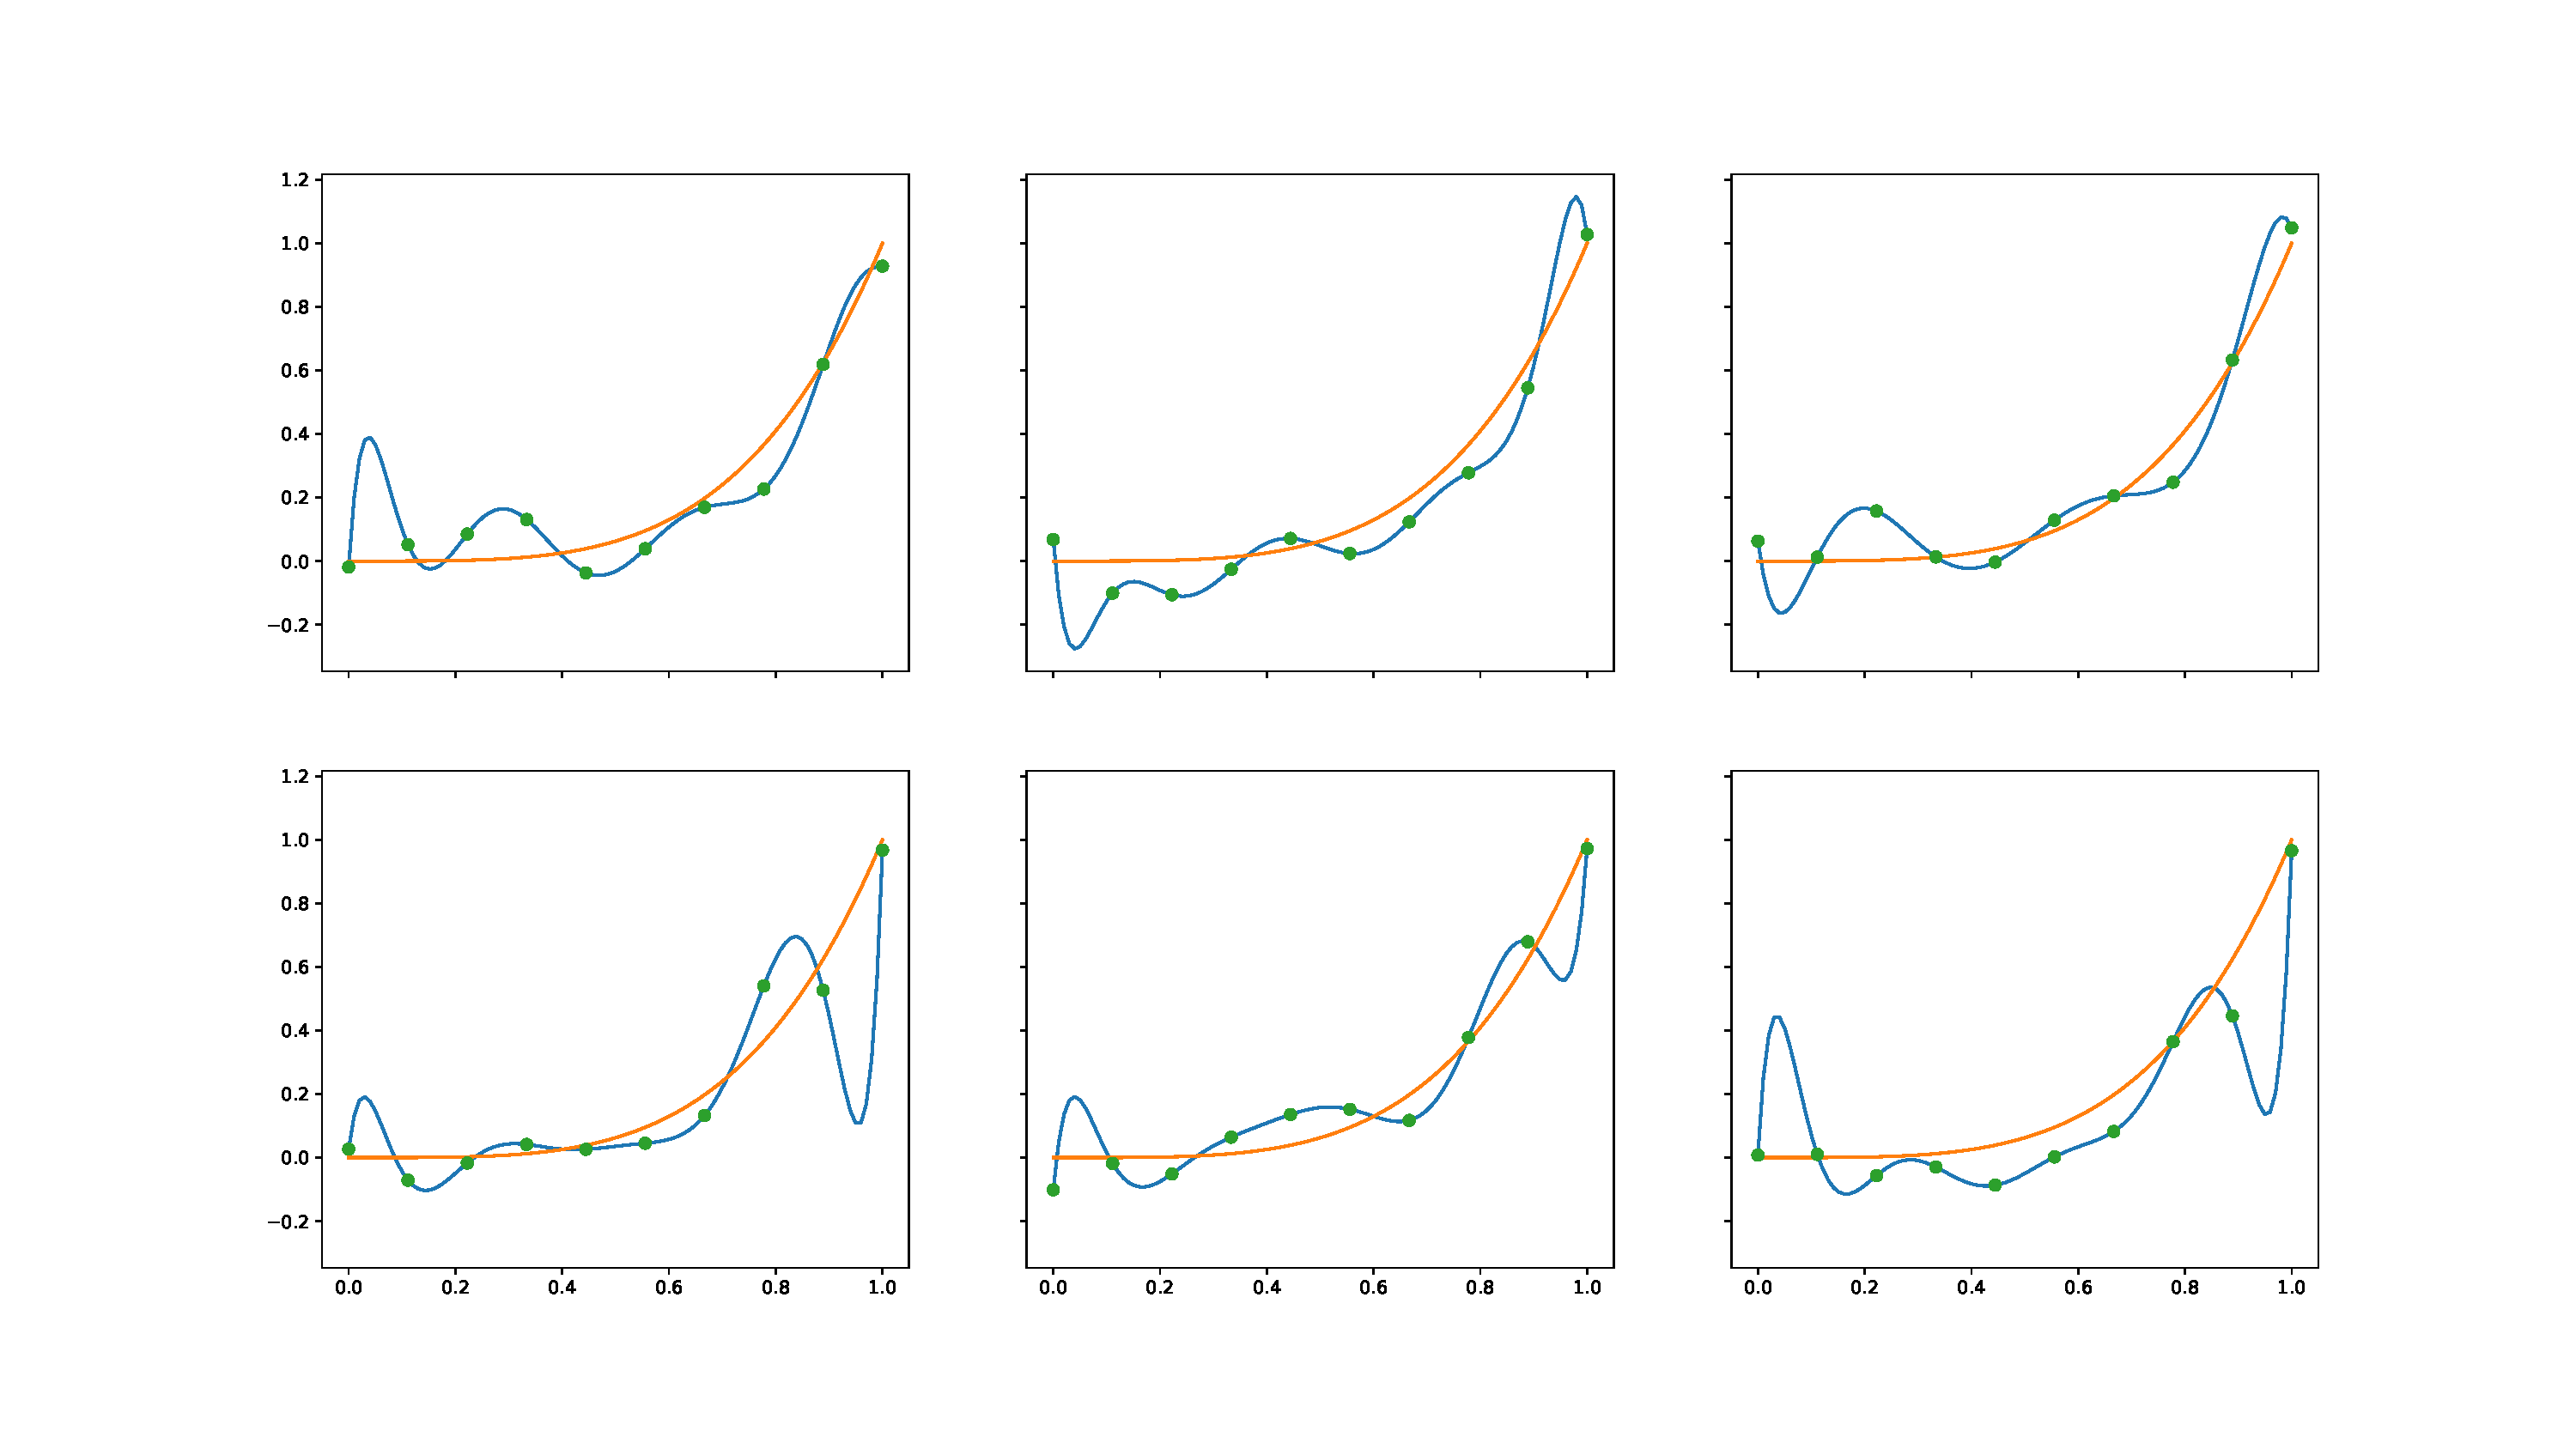
\includegraphics[width=1.0\textwidth]{grid.pdf}
    \caption{\orangeline\; $y=x^4$,\; {\color{green}\textbf{$\bullet$}}\; $y_i = x_i^4 + \text{noise}$,\; \blueline\; polynomial through $(x_i, y_i)$ }    
\end{figure}

\begin{itemize}
    \item You want to ``average away'' the noise. Interpolating noisy data gives wiggly graphs.
    \item large oscillations near left and right endpoints
    \item Increasing size of training set increases model complexity (degree).
\end{itemize}

\section{Bias-variance decomposition}
Let $\hat\theta=\hat\theta(X)$ be an estimator of $\theta$. The \emph{bias of $\hat\theta$} is defined by
\[
    \Bias(\hat\theta,\theta) = \EE\hat\theta - \theta.
\]
The variance of the random variable $\hat\theta$ is given, as usual, by
\[
    \Var \hat\theta = \EE\left[(\hat\theta - \EE\hat\theta)^2\right]
\]
\begin{theorem}[Bias-Variance decomposition]
\[
    \EE\left[(\hat\theta - \theta)^2\right] = \Bias(\hat\theta,\theta)^2 + \Var\hat\theta
\]
\end{theorem}
\begin{proof}
    \begin{align*}
        \EE\left[(\hat\theta - \theta)^2\right] &= \EE\left[(\hat\theta - \EE\hat\theta + \EE\hat\theta - \theta)^2\right]\\
        &= \EE\left[(\hat\theta - \EE\hat\theta)^2\right] 
        + 2\EE\left[(\hat\theta - \EE\hat\theta)(\EE\hat\theta - \theta)\right]
        + \EE\left[(\EE\hat\theta - \theta)^2\right]\\
        &= \Var \hat\theta + \Bias(\hat\theta,\theta)^2,
    \end{align*}
    as
    \[
        \EE\left[(\hat\theta - \EE\hat\theta)(\EE\hat\theta - \theta)\right]
        = (\EE\hat\theta - \theta)\underbrace{\EE[\hat\theta - \EE\hat\theta]}_{=\,0}
        = 0.\qedhere
    \]
\end{proof}
Let $f:\RR\to\RR$ be an unknown function and let $\hat f:\RR\to\RR$ be a known approximation to $f$.
Let $x_0\in\RR$ and suppose that
\[
    Y = f(x_0) + \epsilon,\quad\text{where}\quad \EE[\epsilon]=0.
\]
% Let $\hat f$ be an estimator of $f$.
% The quantities
% \[
%     \EE\left[(\hat f-f )^2\right]\quad\text{and}\quad \EE\left[(\hat f - \EE\hat f)^2\right]
% \]
%  called the \emph{bias} and \emph{variance} of $\hat f$, respectively.
The \emph{squared prediction error} is
 \begin{align*}
     (f(x_0)-\hat f(x_0))^2 &=\EE\left[(\hat f(x_0)- f(x_0))^2\right]\\
     &=\EE\left[(\hat f(x_0)- Y - \epsilon)^2\right]\\
     &= \EE\left[(Y - f + f - \hat f)^2\right]\\
     &= \EE\left[(Y - f)^2\right] 
     + 2\EE\left[(Y - f)(f - \hat f)\right]
     + \EE\left[(f - \hat f)^2\right]\\
     &= \EE[\epsilon^2]
     + 2\epsilon\EE[f - \hat f]
     + \Bias(\hat f, f)
 \end{align*}

 Let $\theta\in\RR$, let $\epsilon$ be a random variable with $\EE[\epsilon]=0$, and let
 \[
     Y = \theta + \epsilon.
\]
Let $\hat\theta$ be an estimator of $\theta$ such that $\hat\theta$ and $\epsilon$ are independent.
\begin{align*}
    \EE[(\hat\theta - Y)^2]
    &= \EE[(\hat\theta - \theta - \epsilon)^2]\\
    &= \EE[(\hat\theta - \EE\hat\theta + \EE\hat\theta - \theta - \epsilon)^2]\\
    &= \EE[(\hat\theta - \EE\hat\theta)^2] 
    + \EE[(\EE\hat\theta - \theta)^2] 
    + \EE[\epsilon^2]
    \\&+ 2\EE[(\hat\theta - \EE\hat\theta)(\EE\hat\theta - \theta)]
    - 2\EE[(\hat\theta - \EE\hat\theta)\epsilon]
    - 2\EE[(\EE\hat\theta - \theta)\epsilon]\\
    &= \Var \hat\theta + \Bias(\hat\theta,\theta) + \Var\epsilon
\end{align*}

We have:
\begin{itemize}
    \setlength\itemsep{0.5em}
    \item $\EE[(\hat\theta - \EE\hat\theta)^2] = \Var \hat\theta$
    \item $\EE\hat\theta - \theta$ is a constant, so
    \begin{align*}
        \EE[(\EE\hat\theta - \theta)^2] &= (\EE\hat\theta - \theta)^2 = \Bias(\hat\theta,\theta)^2,\\
        \EE[(\hat\theta - \EE\hat\theta)(\EE\hat\theta - \theta)] &= \EE[\hat\theta - \EE\hat\theta](\EE\hat\theta - \theta)=0 &\text{(as $\EE[\hat\theta - \EE\hat\theta]=0$),}\\
        \EE[(\EE\hat\theta - \theta)\epsilon] &= (\EE\hat\theta - \theta)
        \EE\epsilon=0&\text{(as $\EE\epsilon=0$).}
    \end{align*}
    \item $\EE[\epsilon^2]=\Var \epsilon$
    \item $\epsilon$ is independent of $\hat\theta$ and, hence, of $\hat\theta-\EE\hat\theta$.
    Therefore,
    \[\EE[(\hat\theta - \EE\hat\theta)\epsilon] = 
    \underbrace{\EE[\hat\theta - \EE\hat\theta]}_{=\,0}\EE\epsilon = 0.\]
\end{itemize}

If you can sample from a distribution, and you have an unbiased estimator, you can learn the parameters of the distribution. The amount of data you need depends on the variance of the estimator.


\section{Notes}

Statistics is the science of the \emph{collection}, \emph{analysis}, and \emph{interpretation} of data. [TPE p.~1]

Data analysis: Oraganization and summarization of data.
Emphasize main features.
Expose underlying structure.
Avoid extraneous assumptions.

Statistical inference:
We postulate that the data are values realized by random variables obeying a probability distribution belonging to some known class, $\cP$.
Typically, $\cP$ is indexed by some \emph{parameter space, $\Theta$}.
\[
    \cP = \{P_\theta : \theta\in\Theta\}
\]
We call the family $\cP$ a \emph{parametric} if $\Theta\subseteq\RR^n$, for some $n$, and \emph{nonparametric}, otherwise.
In statistical inference, we use data to infer (point estimation) a plausible value of $\theta$ or (confidence sets) a subset of $\Theta$ that plausibly contains $\theta$

The estimation problem: Given $g:\Theta\to \RR$ and an $\cX$-valued \emph{random observable} $X$ distributed according to some $P\in\cP$, determine $g(\theta(P))$.
An \emph{estimator} is a function $\delta:\cX\to\RR$. We want to find an estimator $\delta$ such that $\delta(X)\approx g(\theta(P))$.

A \emph{parametric family of distributions} is one that is naturally indexed by a subset $\Theta$ of some Euclidean space $\RR^n$.
The set $\Theta$ is called the \emph{parameter space} of the family. 

Suppose we are given a sample space $\cX\subseteq\RR^p$ and a family $\cP$ of distributions on $\cX$.

Let $X$ be an $\cX$-valued random vector such that $X\sim P$ for some unknown $P\in\cP$.

Using data $x$ realizing $X$ to make draw conclusions about $P$ is called \emph{statistical inference}.

Let $g$ be a \emph{functional} (real-valued function) on $\cP$.

Using data $x$ realizing $X$ to estimate $g(P)$ is called \emph{point estimation}.

Point estimation is a type of statistical inference.
% Using data $x$ realizing $X$ to construct an interval likely to contain $g(P)$ is called \emph{interval estimation}.

Let $P_{\mu,\sigma}$ be the distribution with density
\[
\prod_{i=1}^p\frac1{\sqrt{2\pi}\sigma}e^{-\frac1{2\sigma^2}(x_i-\mu)^2}.
\]
It's the distribution of an \iid sample of size $p$ drawn from $N(\mu,\sigma)$.

Using such a sample to estimate $\mu$ (resp., $\sigma$) is an example of point estimation with
\[
\cX=\RR,\quad \cP=\{P_{\mu,\sigma}\}\quad\text{and}\quad
\text{$g(P_{\mu,\sigma})=\mu$ (resp., $\sigma)$}
\]

A \emph{statistical functional on $\cP$} is a function $g:\cP\to\RR$.
Let $\cP$ be the set of all probability distributions on $\RR$.
For $a\in\RR$, define $$g_a(P)=\int_{-\infty}^adP(x)$$

$$\mu(P)=\int_{-\infty}^\infty x\,dP(x)$$

$$m_k(P)=\int_{-\infty}^\infty (x-\mu(P))^k\,dP(x)$$

Estimating a functional $g:\cP\to\RR$ from data means
constructing a function $\delta:\cX\to\RR$ such that for all distributions $P\in\cP$ and all $\cX$-valued random variables $X\sim P$, the quantity $\delta(X)$ is ``close to'' $g(P)$.
We call $g$ and $\delta$ the \emph{estimand} and \emph{estimator}, respectively.

We must make the descriptor ``close to'' precise if we are to evaluate the quality of an estimator $\delta$ of a functional $g$ in any meaningful way.
The notion of \emph{bias} is a natural interpretation of closeness.
Define
\[
    \Bias(\delta(X), g(P)) = \EE\delta(X) - g(P).
\]
If $\Bias(\delta(X), g(P))<0$ (resp., $\Bias(\delta(X), g(P))>0$), then $\delta(X)$ tends to underestimate (resp., overestimate) $g(P)$.
We say that $\delta(X)$ is an \emph{biased (resp., unbiased) estimator of $g(P)$}
if $\Bias(\delta(X), g(P))\neq0$
(resp., $\Bias(\delta(X), g(P))=0$).


Let $X\sim P\in \cP$.

$$\Bias(\delta(X), g(P))=\EE[\delta(X) - g(P)]$$

Note that if $X\sim P$, then $\EE\delta(X)$ depends only on $\delta$ and $P$ and not on $X$:
\[
    \EE[\delta(X)] = \int_\cX\delta(x)\,dP(x)
\]

Define the \emph{(mean) bias} functional associated to the estimator $\delta$ of $g$,
\[
    \Bias(\delta, g):\cP\lra\RR
\]
by
\[
    P\mapsto\Bias_P(\delta, g) := \EE[\delta(X)] - g(P),
\]
where $X$ is any $\cX$-valued random variable such that $X\sim P$.

$\delta$ is an unbiased estimator of $g$ if and only if $\Bias(\delta, g)$ is an unbiased estimator of the zero functional.

Mean bias vs.\ median bias. Exercise?
\end{document}